\documentclass[a4paper, 12pt]{ltjsarticle}
\usepackage{thesis}

% 表紙のスタイル設定
\newcommand{\coverpage}{
\begin{titlepage}
\begin{center}
\vspace*{1.5cm}

{\LARGE 2024年度卒業論文}\\[2cm] % 年度タイトル

{\Huge {常微分方程式のシミュレータ教材の開発}}\\[4cm] % 論文タイトル 二行にしたい場合はバックスラッシュ2個つける

{\LARGE 指導教員 須田 宇宙 准教授}\\[2cm] % 指導教員名
{\LARGE 千葉工業大学 情報ネットワーク学科}\\[0.5cm] % 学科名

{\LARGE 須田研究室}\\[2.5cm] % 研究室名

{\LARGE {2032144} 氏名 {山﨑亮輔}} \\[1.5cm] % 学番と名前

\vfill
\end{center}

% 提出日を右下に配置
\begin{flushright}
{\LARGE 提出日 \textnormal{2025年01月17日}}\\[1.5cm] % 提出日
\end{flushright}

\vfill
\end{titlepage}
}

\begin{document}

% 表紙の挿入
\coverpage

\tableofcontents

\clearpage

\section{緒言}
\clearpage
\section{シミュレータ教材について}
理工学系の教育現場では,不可視現象を取り扱うことがある.不可視現象を取り扱う分野の学習に関して,座学のみでは高い学習効果を得ることが難しい.そのため,e-Learningコンテンツとして不可視現象をデジタル端末で可視化,可聴化する教材であるシミュレータ教材を用いた体験的な学習が有効的である.シミュレータ教材は目的に応じて次のように分類することができる.
\begin{enumerate}
\item 汎用測定機器教材\\
入力データを与えることで,一般の測定機器のように解析を行わせることを目的としている.
\item 時間変化を伸縮する教材\\
高速あるいは低速で時間変化する現象を伸縮して可視化することを目的としている.
\item 3D-CG表示教材\\
二次元の図では断片的に表すのみの現象を,3D-CGの技法を取り入れることで立体的に表現し,あらゆる角度から観察できる教材にすることを目的としている.
\item 可聴化教材\\
視覚では確認が難しい音響現象音響現象を,聴覚的に合成音で確認することを目的している.
\item 現象のアニメーション化\\
シミュレーション結果をもとに,直感的,現実的なアニメーション技法に基づきビットマップ対応で表現することを目的としている.
\end{enumerate}
\clearpage
\section{シミュレーションについて}
\subsection{概要}
シミュレーションとは,自然現象や社会現象を方程式によって表現し,あるケースにおいての変化を計算することである.現実世界で実験を行うことが困難な現象について,コンピュータ上で仮想的な環境を構築し,条件を変更しながら実験を行うことによって,現象の本質を理解したり予測をすることができる.また,シミュレーションは幅広い分野で活用されており,私たちの生活をより豊かにする上で重要な役割を果たしている.
\subsection{流れ}
シミュレーションの流れは次のようになる.
\begin{enumerate}
\item モデル化\\
ある現象を法則に沿った方程式にする.
\item プログラミング\\
モデル化したものをコンピュータで計算処理するためのプログラミングを行う.
\item 計算の実行\\
プログラムを実行し,シミュレーションを行う.
\item 結果の分析\\
結果から条件を変更し再計算を行なったり,結果を分析し結論を導く.
\end{enumerate}
\subsection{誤差}
シミュレーションにおいて誤差が生じる.この誤差が生じる原因としては,以下の3つがある.
\begin{enumerate}
\item モデル化\\
現実世界の現象の要素を全て正確にモデル化することはできないため.
\item 打ち切り誤差\\
連続的な現象を離散化することでコンピュータで計算を行っているため.
\item 丸め誤差\\
コンピュータでの小数点表現は有限桁のため表現できない数が存在するため.
\end{enumerate}
また,

\section{常微分方程式について}
\subsection{概要}
未知の関数とその導関数との関係を表す方程式を微分方程式といい,1つの変数で導関数が表されている微分方程式を常微分方程式という.シミュレーションで用いられる際には時間を変数とすることが多い.
\subsection{数値解法}
常微分方程式の数値解法は初期値問題に分類され,与えられた導関数における微小区間の面積を原関数における微小区間の変化分として原関数を求められる.連続的なグラフを離散的に数値を求め,その点を結びグラフを描くため誤差が生じる.代表的な解法としてオイラー法と4次ルンゲクッタ法がある.以下は1階常微分方程式の各解法である.
与えられた導関数を$\frac{dy}{dx}=f(x,y)$,初期値を$(x,y)=(x_0,y_0)$,微小区間の幅を$h$とする.
\subsection{オイラー法}
オイラー法では,現在の点における傾きから次の点を予測していく方法である.現在の点を$(x_n,y_n)$とすると,$(x_{n+1},y_{n+1})$は以下のようになる.
\begin{equation}
  x_{n+1}=x_n+h
\end{equation}
\begin{equation}
  y_{n+1}=y_n+hf(x_n,y_n)
\end{equation}
精度については,局所誤差は$O(h^2)$,大域誤差は$O(h)$である.
\clearpage
\subsection{4次ルンゲクッタ法}
4次ルンゲクッタ法では,次の補正値$k$を用いて次の点を求める.
\begin{equation}
  k_1=hf(x_n,y_n)\label{eq:3}
\end{equation}
\begin{equation}
  k_2=hf(x_n+\frac{h}{2},y_n+\frac{k_1}{2})\label{eq:4}
\end{equation}
\begin{equation}
  k_3=hf(x_n+\frac{h}{2},y_n+\frac{k_2}{2})\label{eq:5}
\end{equation}
\begin{equation}
  k_4=hf(x_n+h,y_n+k_3)\label{eq:6}
\end{equation}
\eqref{eq:3}では,現在の点を用いており,\eqref{eq:4}と\eqref{eq:5}は現在の点と次の点の中点を用いている.最後に,\eqref{eq:6}では,次の点を用いている.
現在の点を$(x_n,y_n)$とすると,$(x_{n+1},y_{n+1})$は以下のようになる.
\begin{equation}
  x_{n+1}=x_n+h
\end{equation}
\begin{equation}
  y_{n+1}=y_n+\frac{1}{6}(k_1+2k_2+2k_3+k_4)
\end{equation}
また,局所誤差は$O(h^5)$,大域誤差は$O(h^4)$である.
\clearpage
\section{開発したシミュレータ教材について}
\subsection{目的}
本研究では,常微分方程式の数値解法を学ぶ際に,実際のシミュレーションにおける初期値の扱い方との乖離による疑問を解決することを目的とし,特に,微小区間の幅を自ら設定させることを理解させる教材を開発することである.
\subsection{使用方法}
シミュレータ教材の画面を図\ref{fig:シミュレータ教材の画面}に示す.①の操作部でシミュレーションをする導関数と初期値を選択し,Startボタンを押すことで,②ではオイラー法によるグラフと理論値のグラフを視覚的に確認できる.また,③では誤差が最大となる部分のグラフをより視覚的に確認できる.④では計算回数,誤差,必要な精度を満たしているのかの判定文を確認できるようにしている.

\begin{figure}[h]
\begin{center}
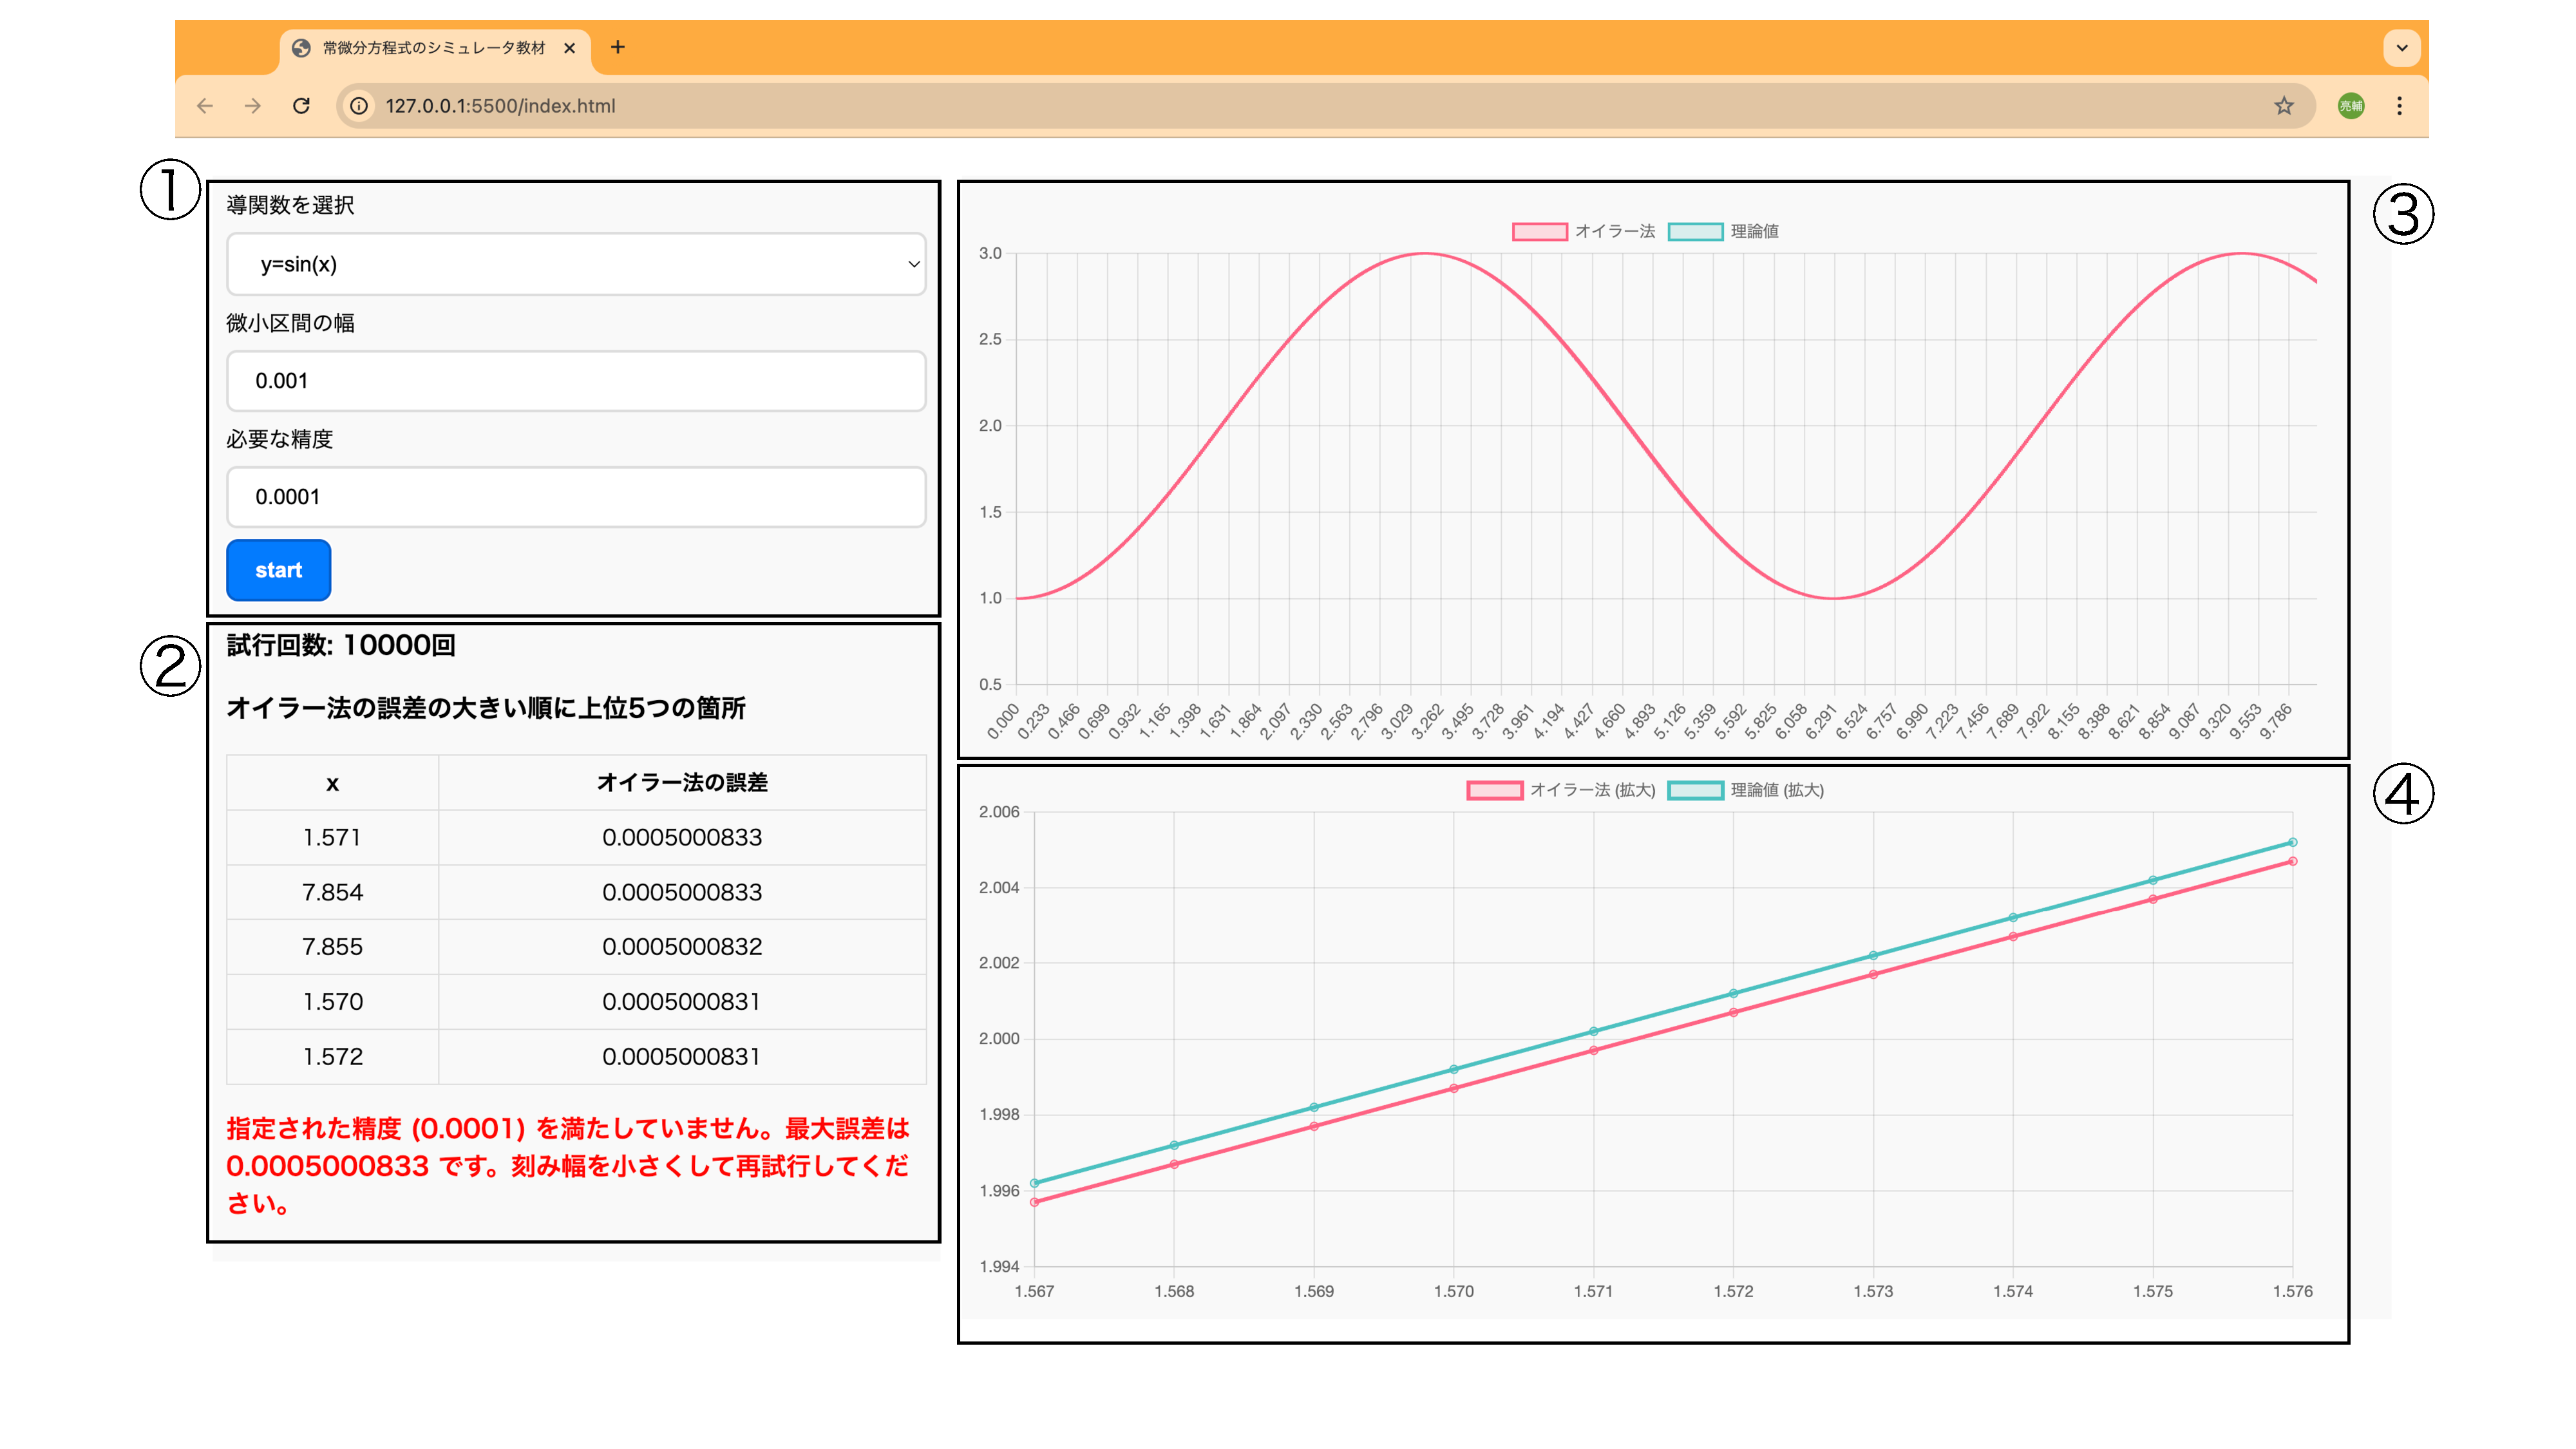
\includegraphics[clip,width=\textwidth,keepaspectratio]{sim-image.pdf}
\end{center}
\caption{シミュレータ教材の画面}
\label{fig:シミュレータ教材の画面}
\end{figure}

\clearpage
\subsection{使用例}
本研究で開発したシミュレータ教材は常微分方程式の基礎的な知識を持っている前提で演習問題を解く際の補助教材として使用することを想定している.また,演習問題として,"導関数を$\sin(x)$において必要な精度が0.01未満となるには微小区間の幅をいくつに設定すれば良いか."について解くことを想定した例を示す.図\ref{fig:シミュレータ教材を開いた際の画面}は開発した教材を開いた際の画面である.図\ref{fig:シミュレータ教材を開いた際の画面}から導関数や微小区間の幅を設定してシミュレーションをすることができる.

\begin{figure}[h]
\begin{center}
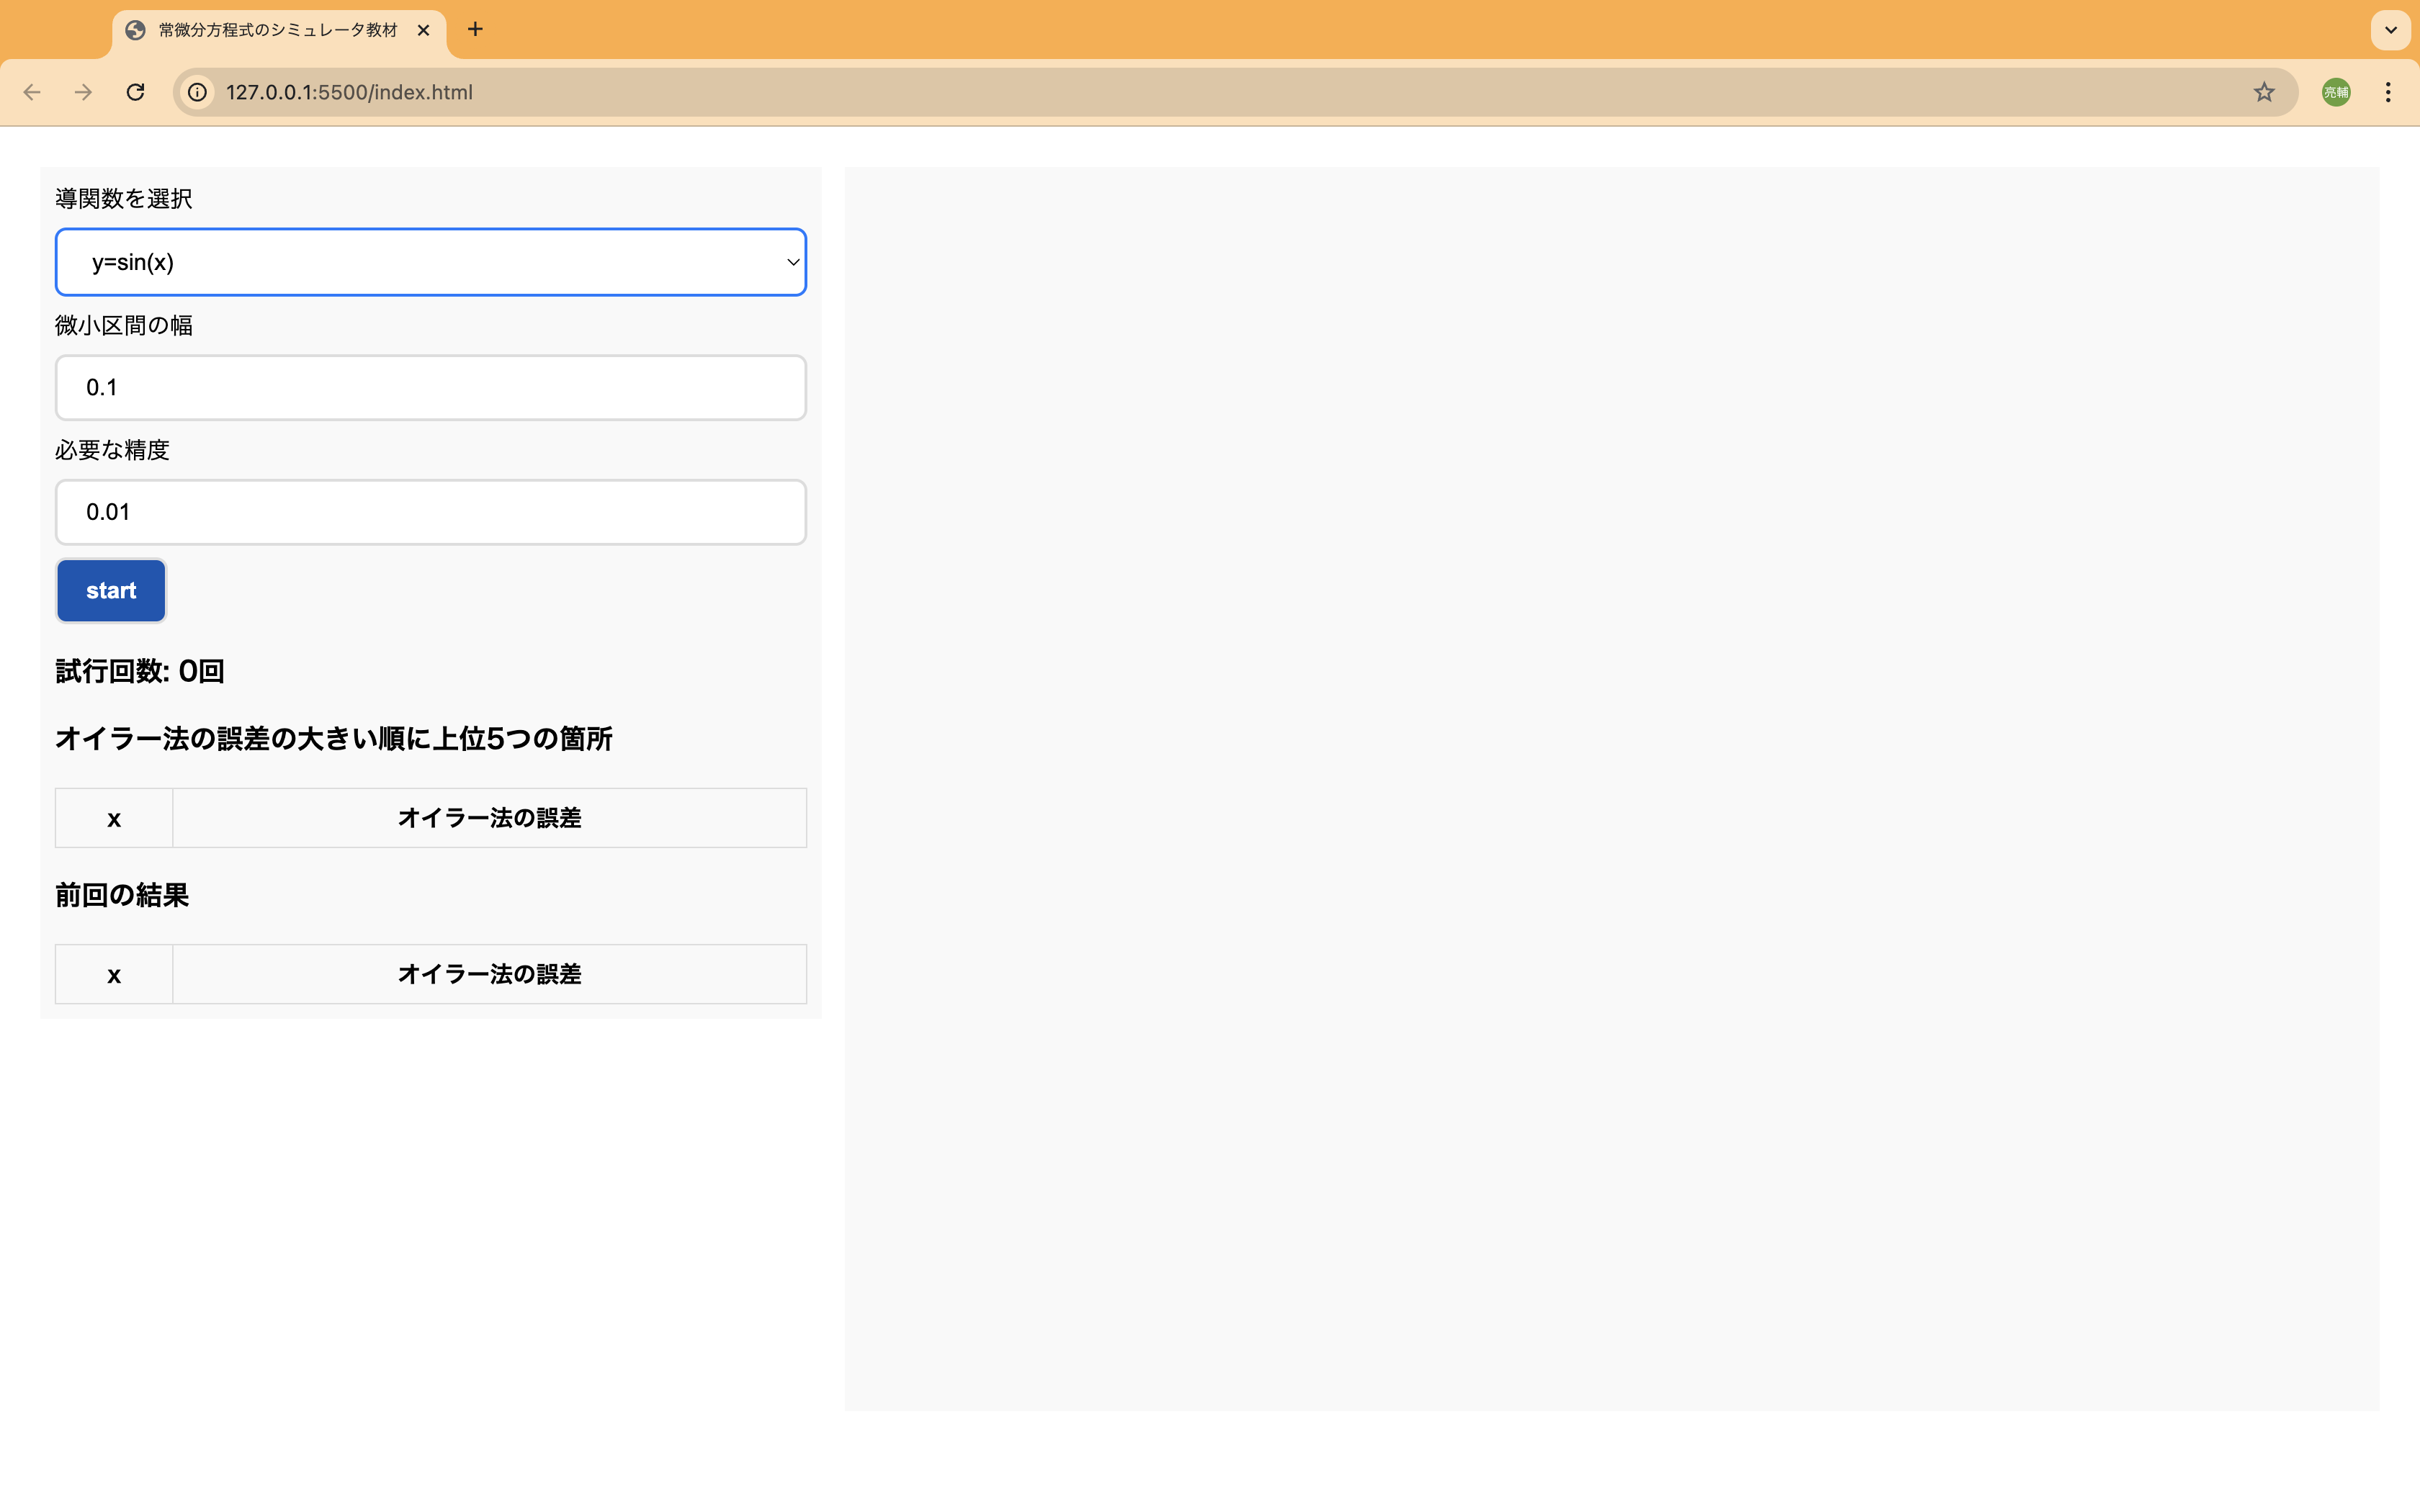
\includegraphics[clip,width=\textwidth,keepaspectratio]{sim-sample1.png}
\end{center}
\caption{シミュレータ教材を開いた際の画面}
\label{fig:シミュレータ教材を開いた際の画面}
\end{figure}

\clearpage

まず,本教材を用いた演習の例について記述していく.導関数に$\sin(x)$,微小区間の幅を0.1,必要な精度を0.01を設定してStartボタンを押した際の画面を図\ref{fig:シミュレータ教材の使用例1}に示す.計算が完了すると結果部分,グラフ描画部分及び拡大グラフ描画部分が表示される.

\begin{figure}[h]
\begin{center}
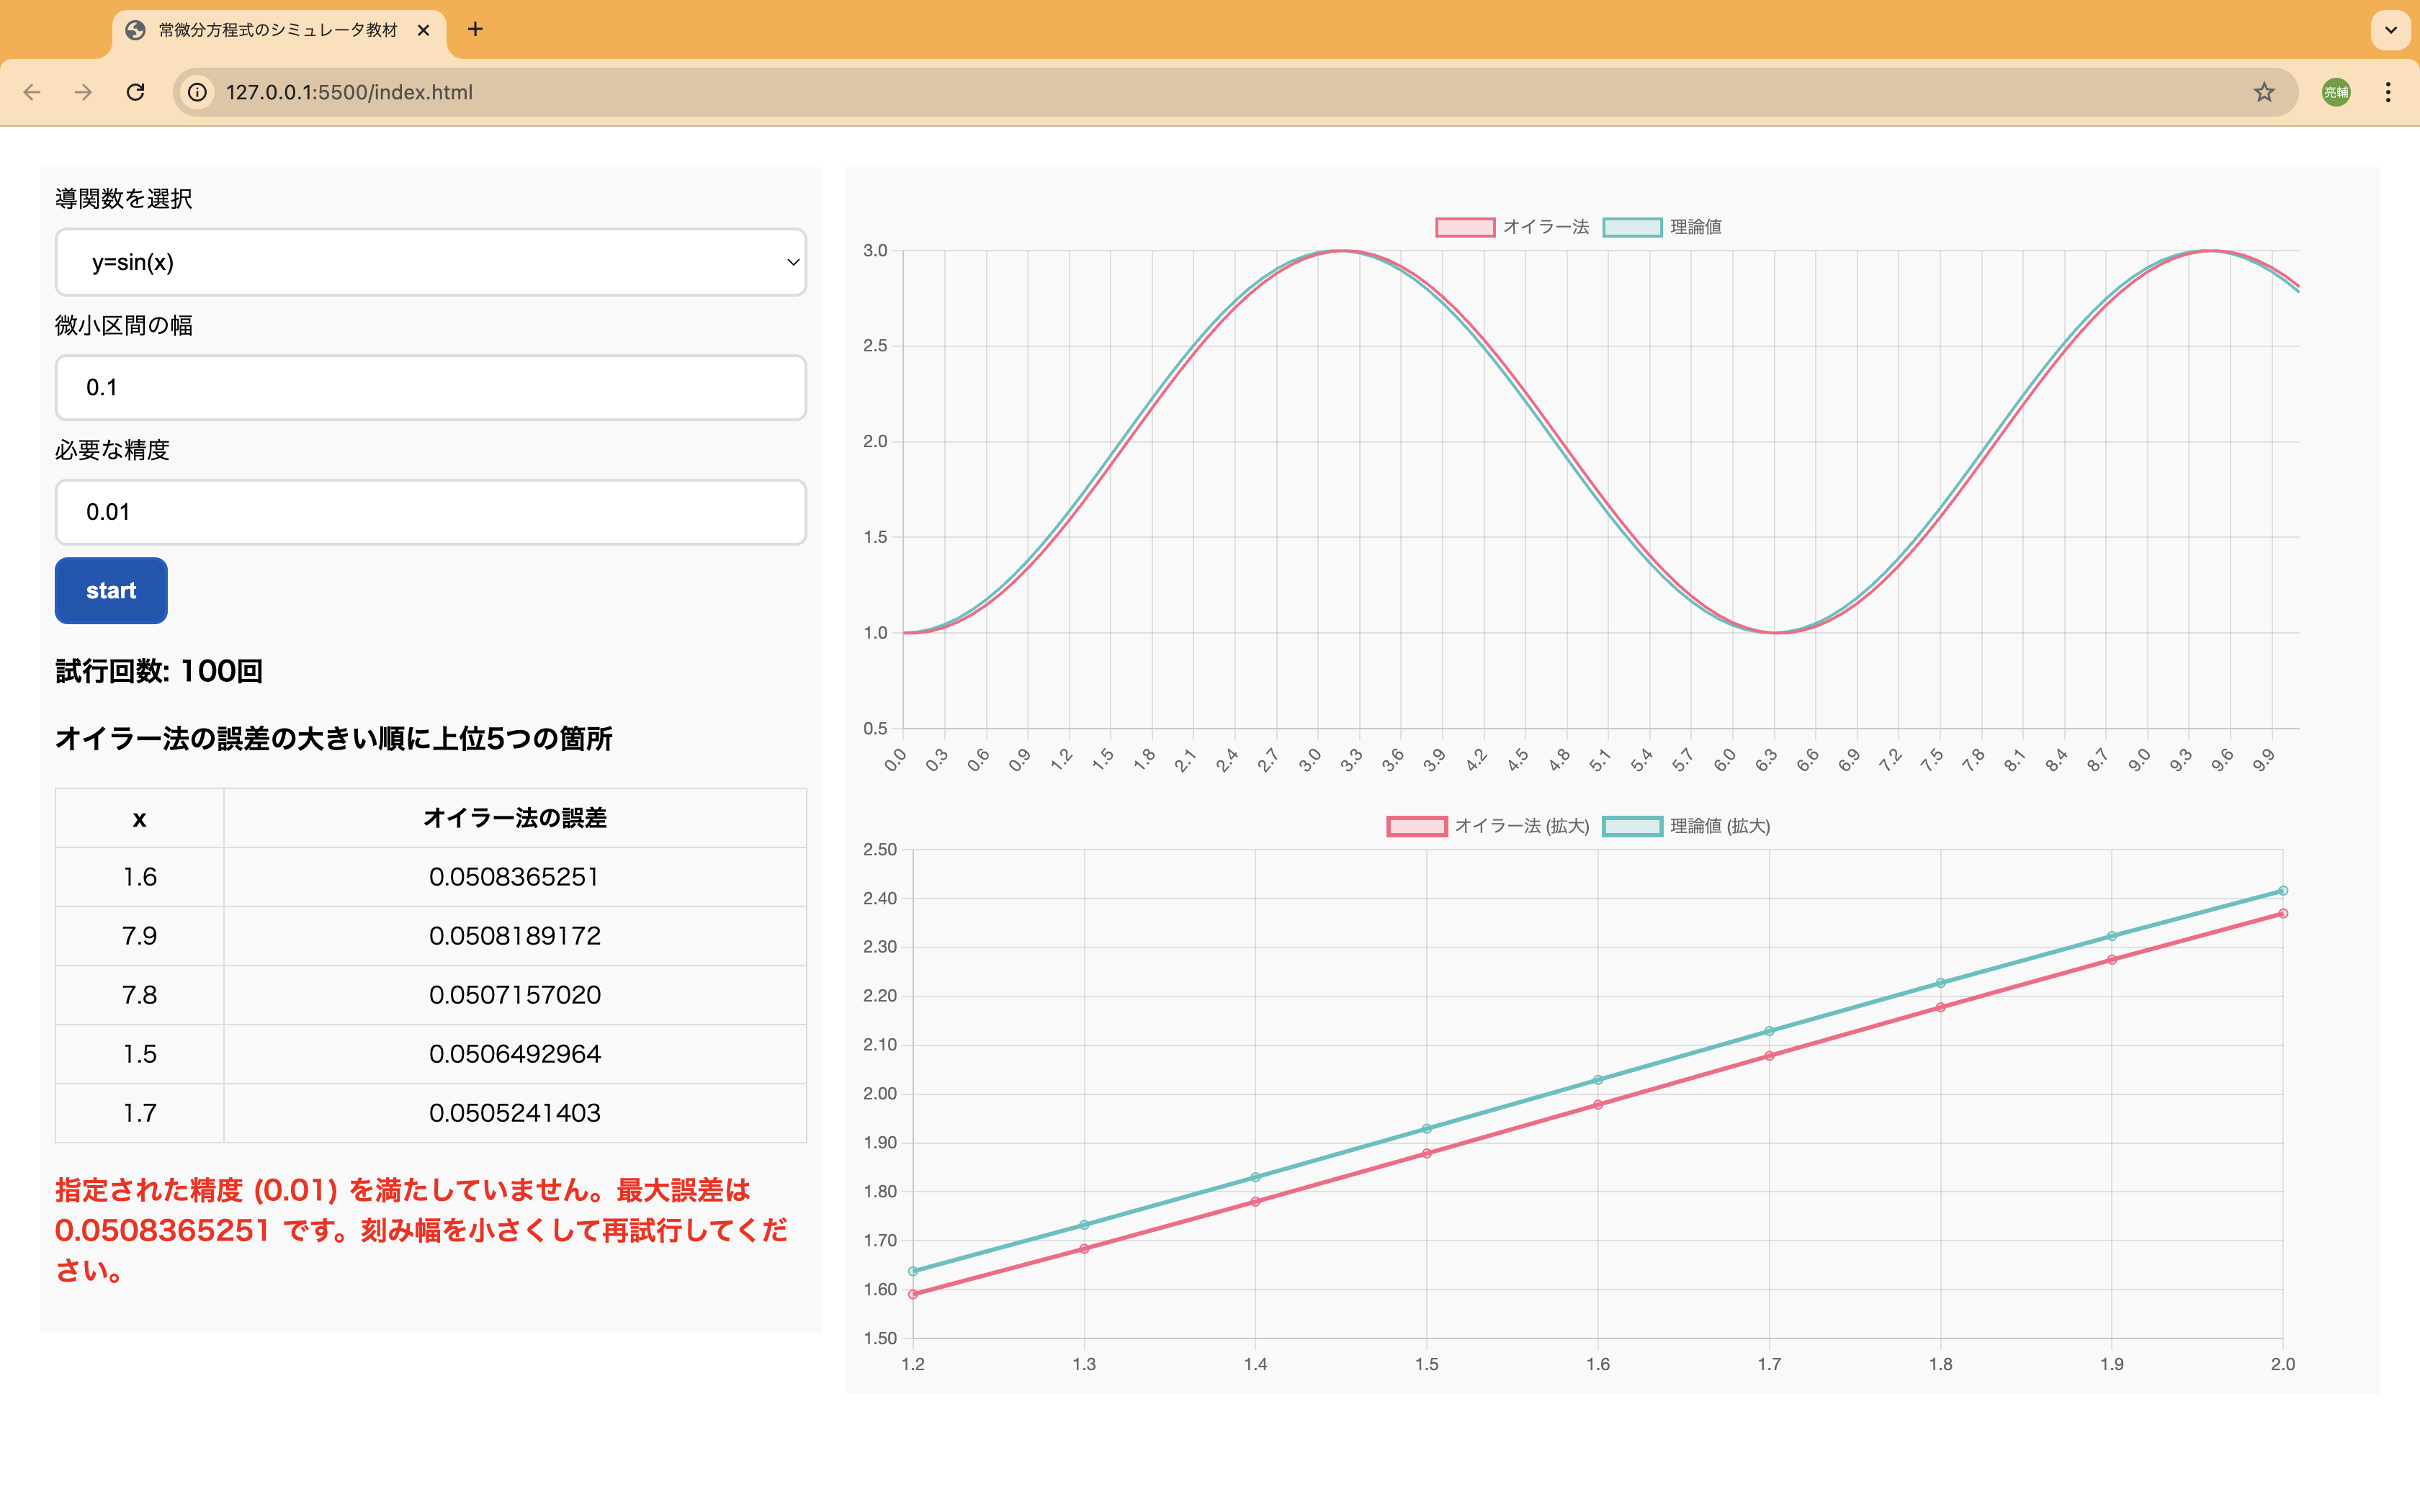
\includegraphics[clip,width=\textwidth,keepaspectratio]{sim-sample2.png}
\end{center}
\caption{シミュレータ教材の使用例1}
\label{fig:シミュレータ教材の使用例1}
\end{figure}

\clearpage

次に,必要な精度を満たしていないため微小区間の幅を0.01に変更してStartボタンを押した際の画面を図\ref{fig:シミュレータ教材の使用例2}に示す.結果部分から必要な精度を満たすようになったのがわかる.ここから,導関数$\sin(x)$は微小区間の幅が0.01であれば誤差を0.01より小さくすることができることがわかる.

\begin{figure}[h]
\begin{center}
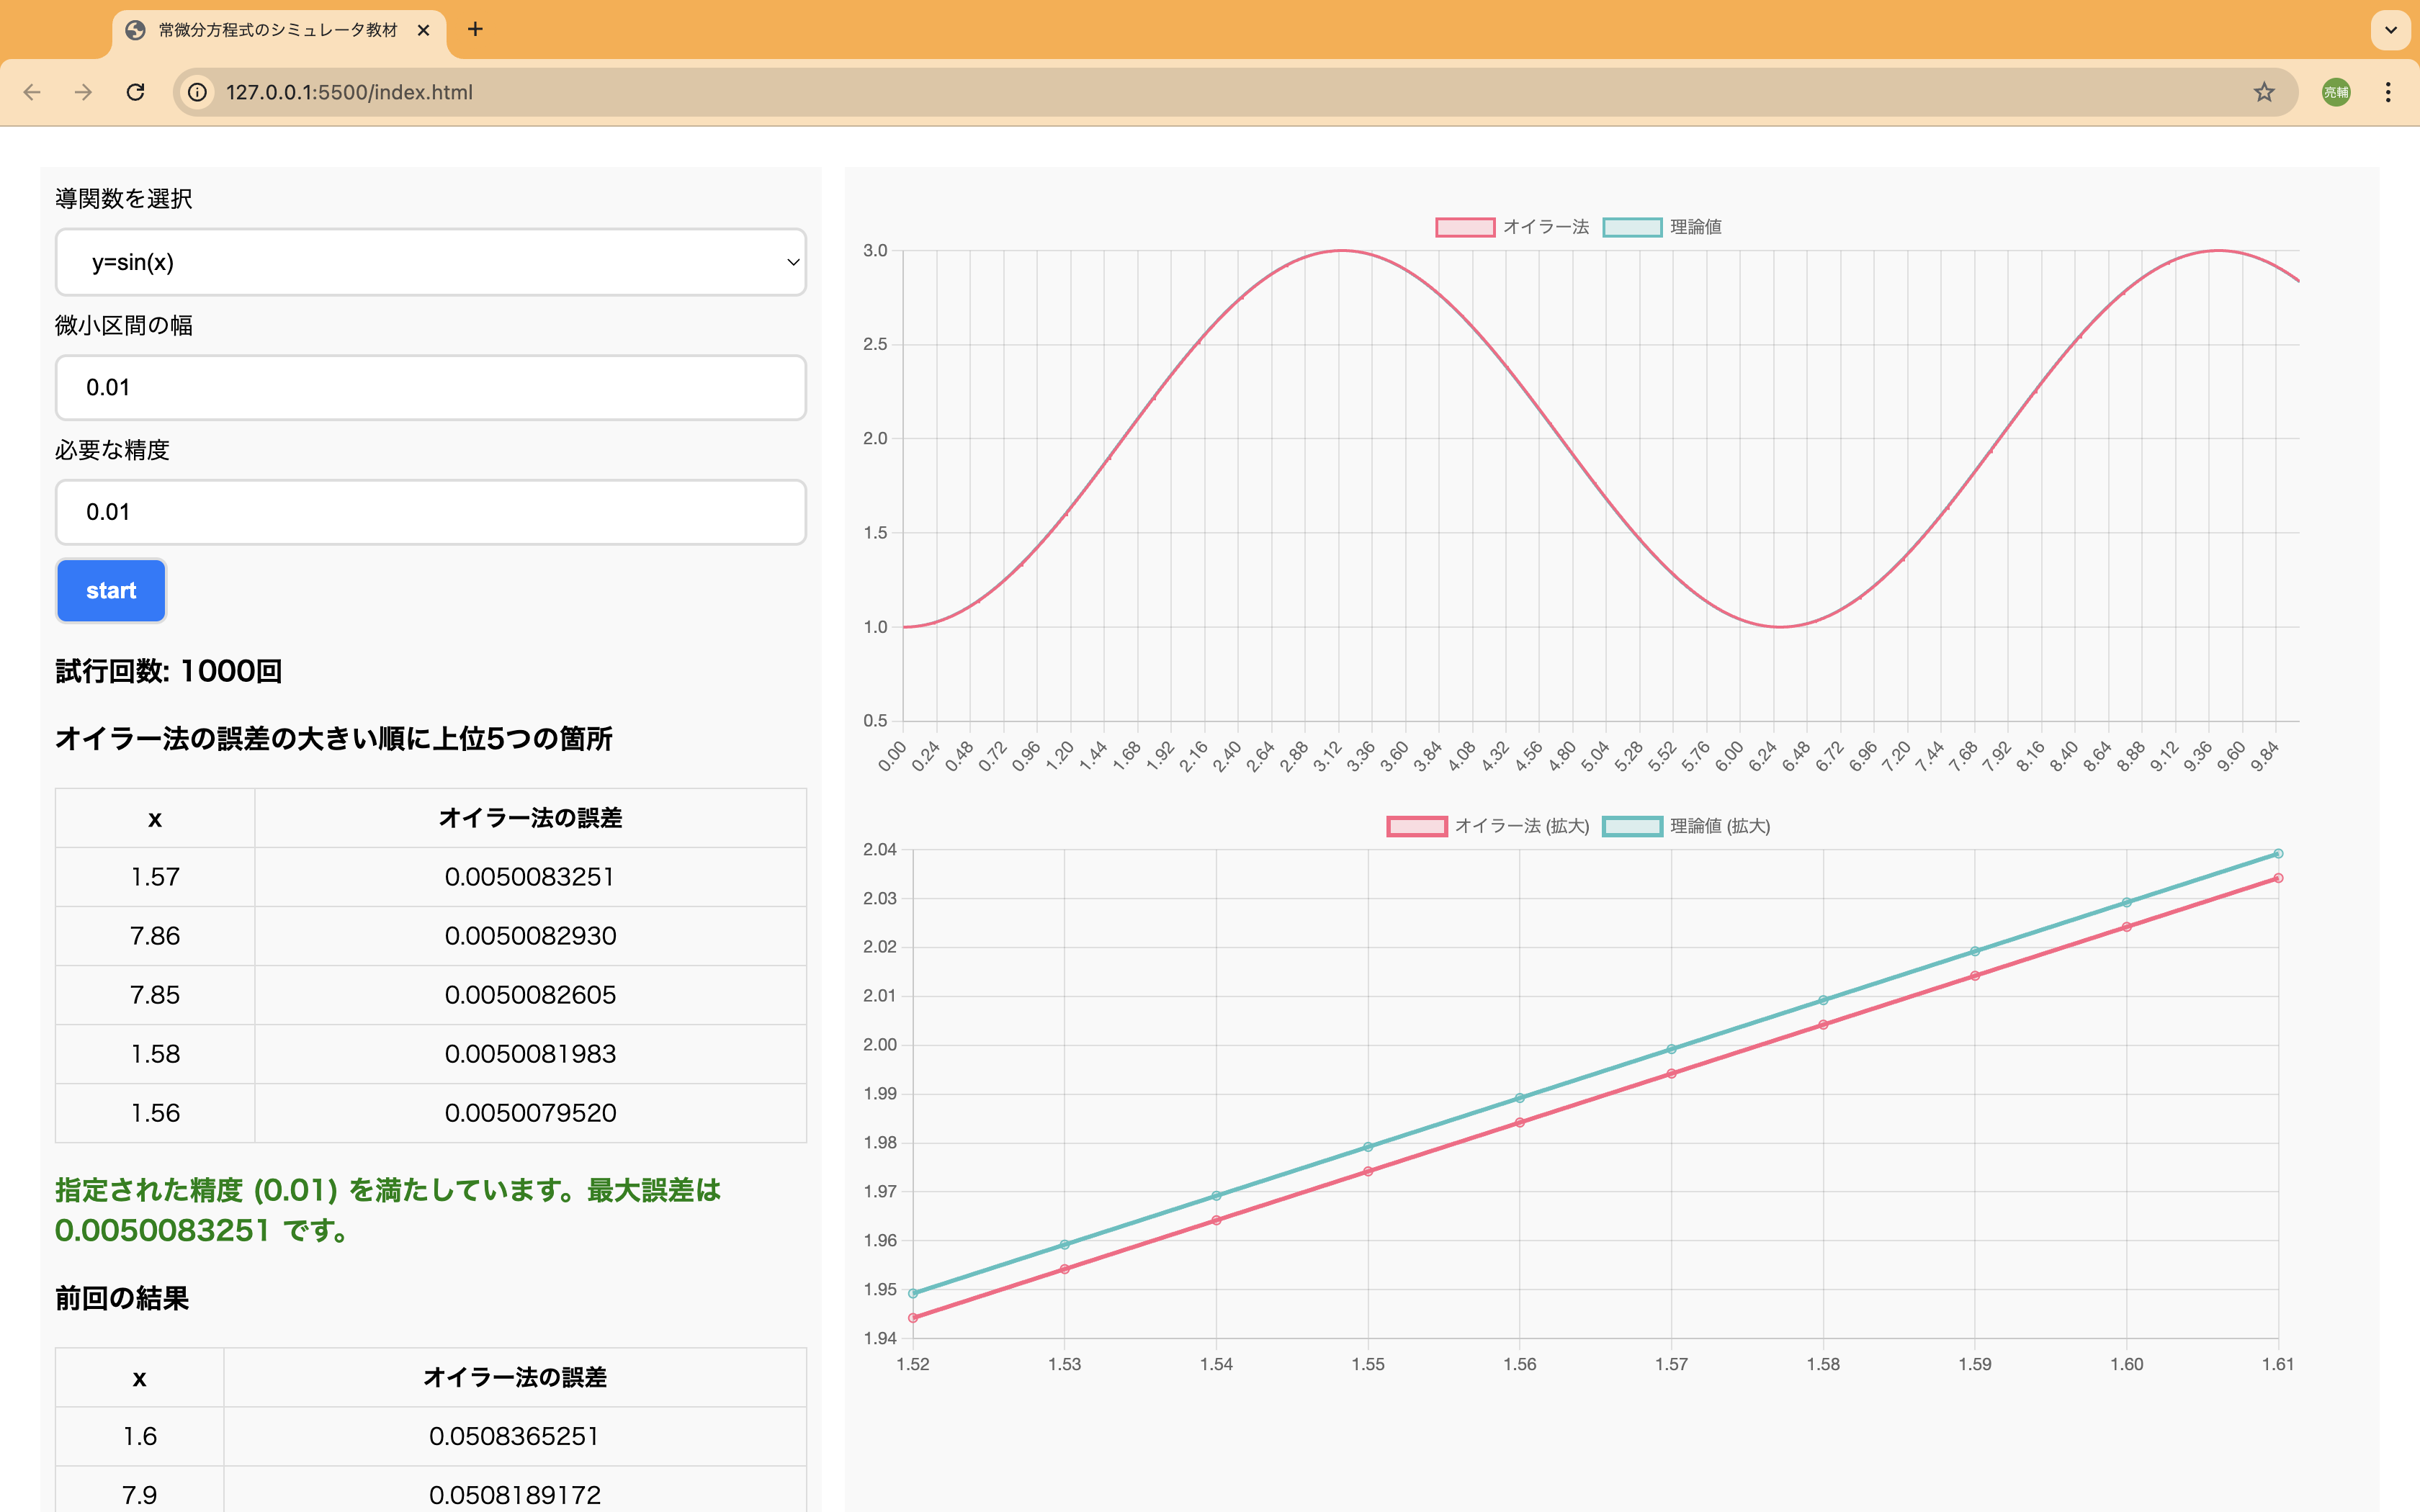
\includegraphics[clip,width=\textwidth,keepaspectratio]{sim-sample3.png}
\end{center}
\caption{シミュレータ教材の使用例2}
\label{fig:シミュレータ教材の使用例2}
\end{figure}

\clearpage

最後に,微小区間の幅を0.02に変更してStartボタンを押した際の画面を図\ref{fig:シミュレータ教材の使用例3}に示す.結果部分から必要な精度を満たしていないことがわかる.ここから,導関数$\sin(x)$は微小区間の幅が0.02の際は,誤差が0.01を超えることがわかる.そのため,演習問題の回答は0.01となる.

\begin{figure}[h]
\begin{center}
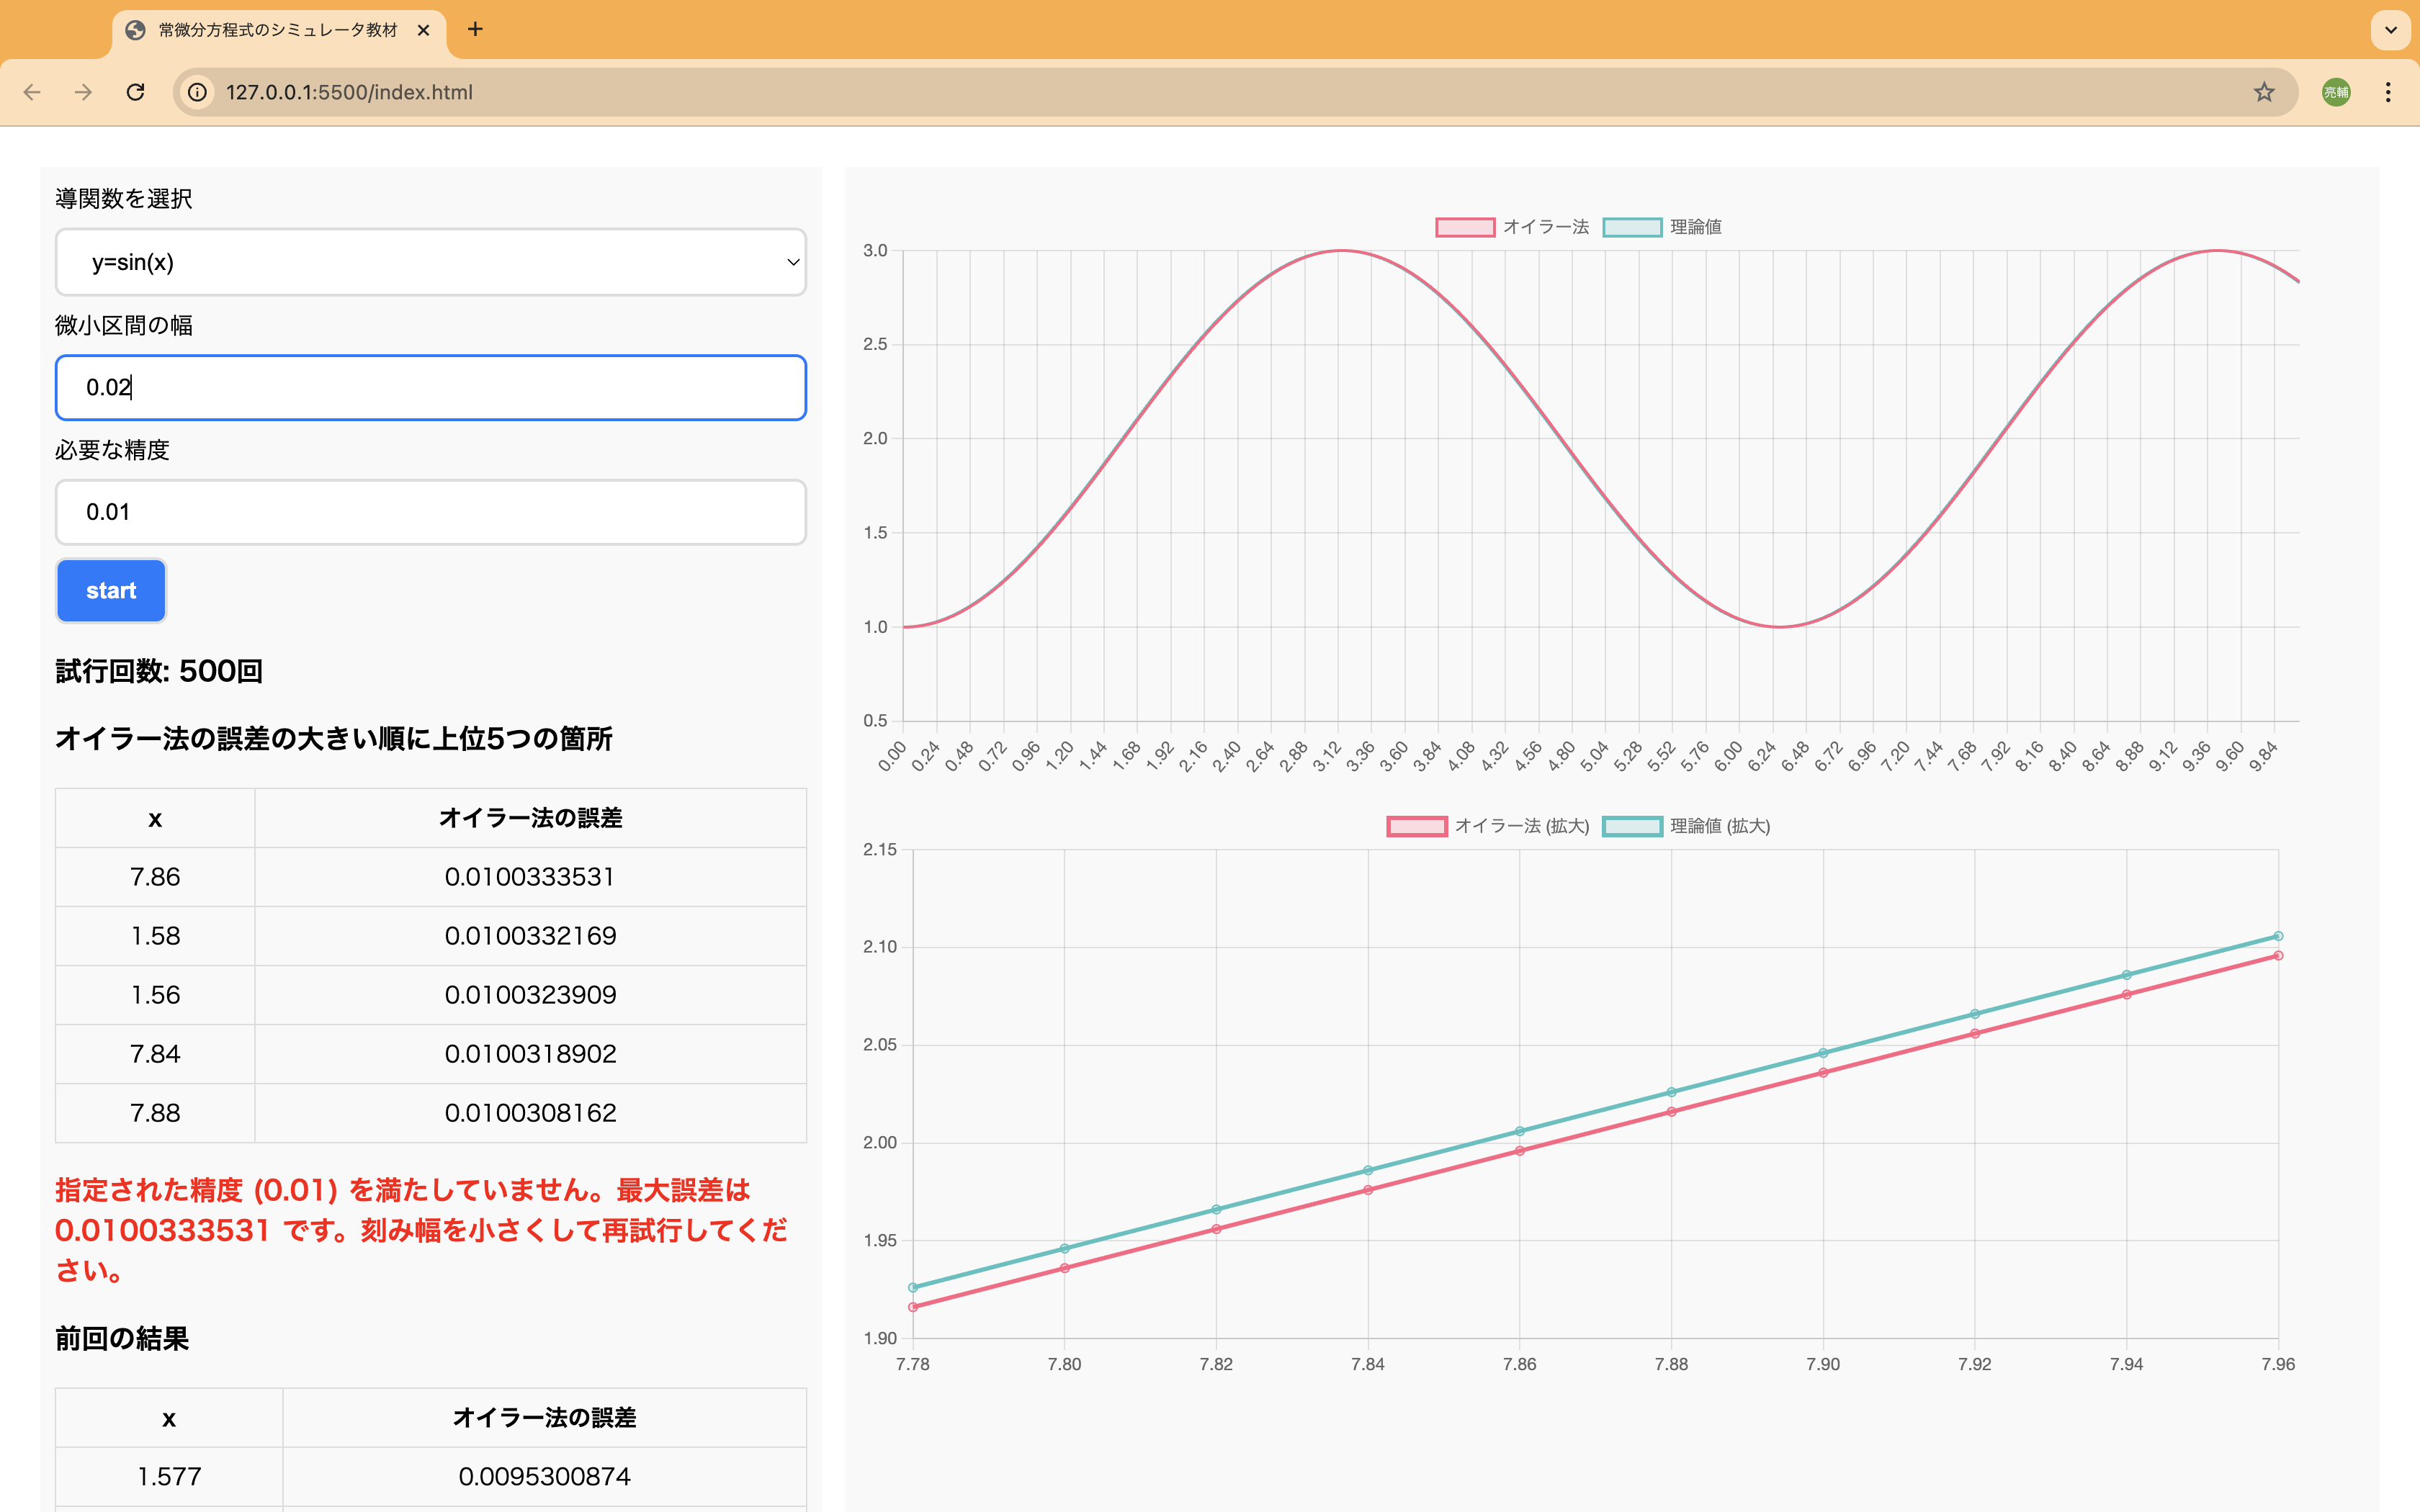
\includegraphics[clip,width=\textwidth,keepaspectratio]{sim-sample4.png}
\end{center}
\caption{シミュレータ教材の使用例3}
\label{fig:シミュレータ教材の使用例3}
\end{figure}

\section{教材の実装について}
\subsection{開発言語}
\subsubsection{HTML}
HTMLとは,Webの最も基本的な構成要素であり,Webページを作成する際に使用されるマークアップ言語である.また,正式名称はHyper Text Markup Language(ハイパーテキストマークアップランゲージ)である.HTMLの特徴としては,ハイパーテキスト機能でWebページから別のWebページに簡単に遷移することができる点である.
\subsubsection{CSS}
CSSとは,主にHTMLで記述された文書の体裁や見栄えを表現するためのスタイルシート言語である.また,正式名称はCascading Style Sheets(カスケーディングスタイルシート)である.
\subsubsection{JavaScript}
JavaScriptとは,主にWebページで使用されている,インタープリンター型の第一級関数を備えたプログラミング言語である.また,プロトタイプベースで動的な言語のため,オブジェクト指向,命令型,宣言型といったスタイルに対応している.
\subsubsection{Chart.js}
Chart.jsとは,JavaScriptアプリケーション開発向けのチャート作成ライブラリの一つである.オプションが豊富で視認性の良いグラフを作成することができる.今回採用した理由として,2013年に作成され,現在もアップデートが行われており,GitHubスター数は約6万,npmダウンロード数は毎週約240万と人気のあるライブラリであると判断したためである.
\clearpage
\subsection{実装機能}
\subsubsection{操作部分}
シミュレータ教材の操作部分を図\ref{fig:操作部分}に示す.導関数の選択は$-2x$,$\sin(x)$及び$\sin(x)\cos(x)-y$の3つのグラフを用意した.微小区間の幅は1から0.0001の範囲で,必要な精度は0.1から0.00001の範囲で入力できるようになっている.Startボタンを押した際に選択されている条件で計算をすることができる.

\begin{figure}[h]
\begin{center}
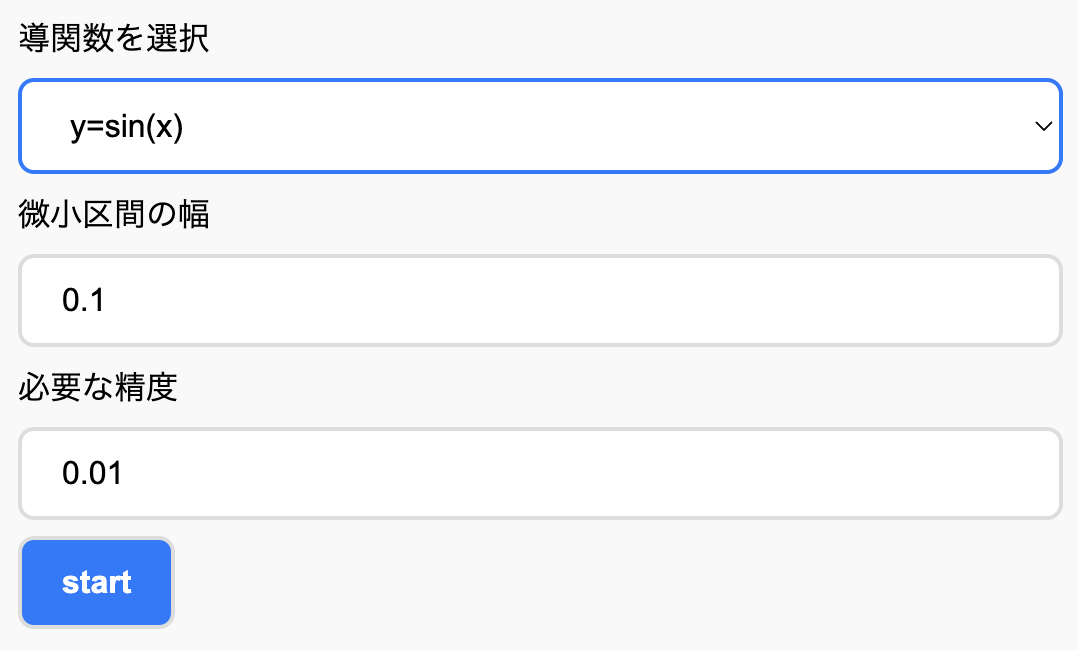
\includegraphics[clip,width=\textwidth,keepaspectratio]{sim-sousa.png}
\end{center}
\caption{操作部分}
\label{fig:操作部分}
\end{figure}

\subsubsection{結果部分}
結果部分を図\ref{fig:結果部分}に示す.結果部分はシミュレーションをする範囲の最大と微小区間の幅の商を計算コストとし,それを表示する試行回数,オイラー法によって計算された数値のと理論値の差を誤差とし,誤差の大きい順に5つの$x$の値と誤差の表,操作部分で入力された必要な精度を満たしているかの判定文及び再計算を行なった際に前回の計算の誤差の大きい順に5つの$x$の値と誤差の表を表示した.精度の判定は満たしている際は緑色の文字で,そうでない際は赤色で表示することでわかりやすくしている.ここでは微小区間の幅を変更することによって誤差がどの程度変化したかを数値で確認することができる.

\begin{figure}[h]
\begin{center}
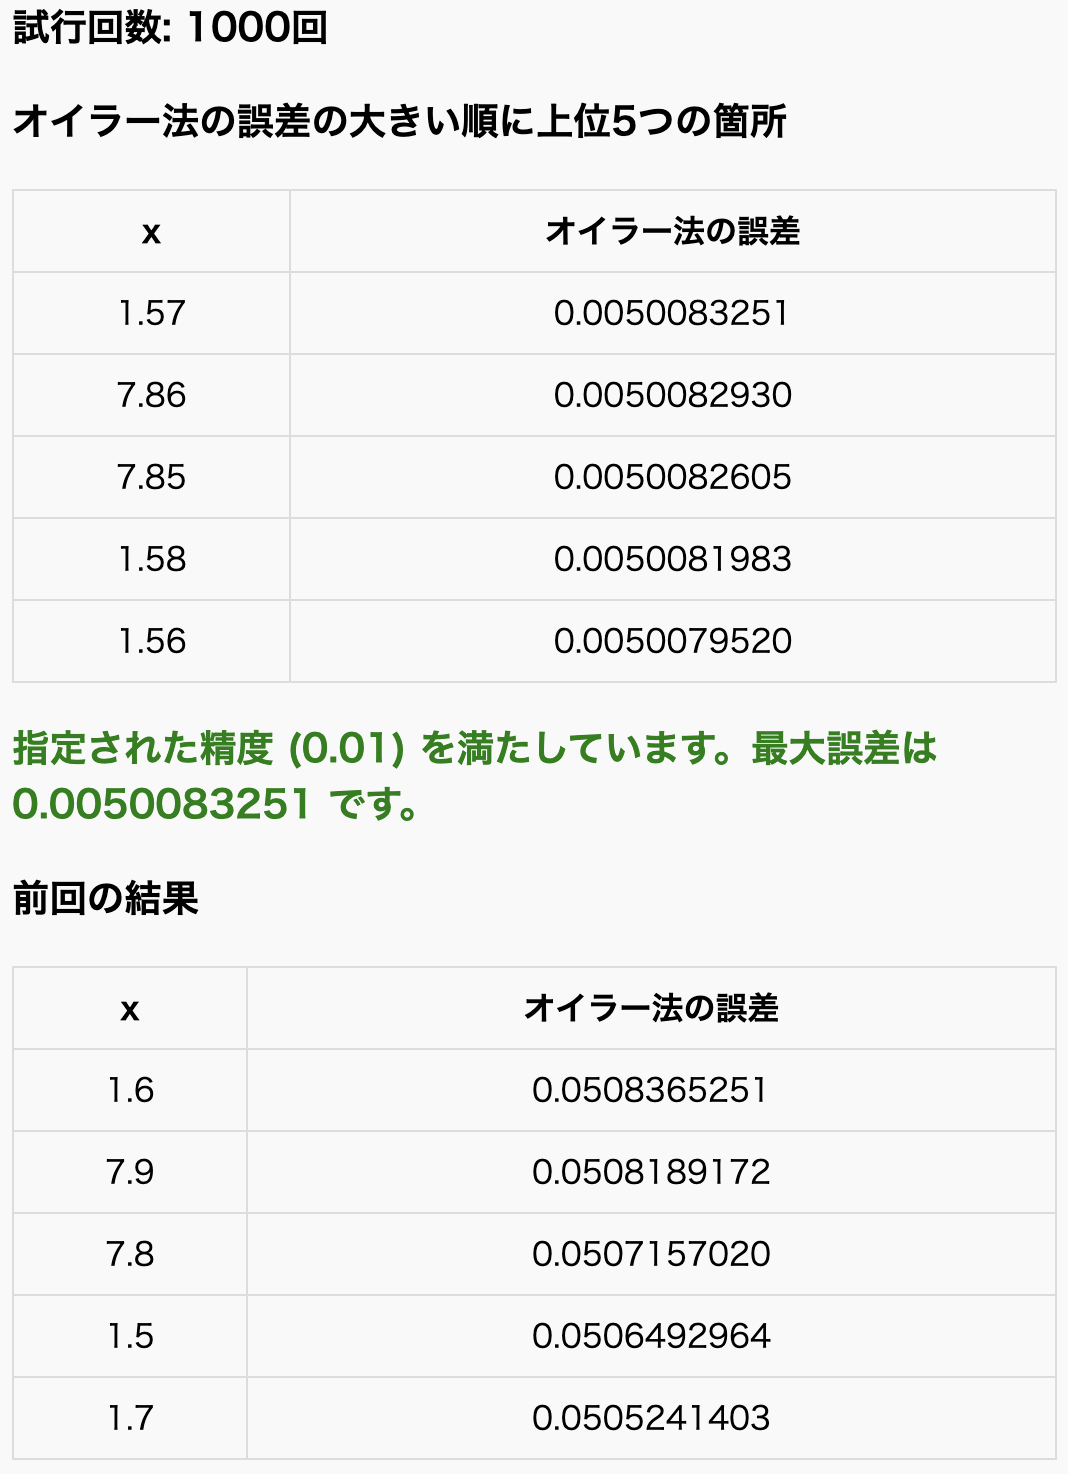
\includegraphics[clip,width=0.7\textwidth,keepaspectratio]{sim-kekka.png}
\end{center}
\caption{結果部分}
\label{fig:結果部分}
\end{figure}

\clearpage

\subsubsection{グラフ描画部分}
グラフ描画部分を図\ref{fig:グラフ描画部分}に示す.計算が完了するとグラフが描画され,オイラー法は赤色のラインで,理論値は緑色のラインで表現している.理論値のラインを背面にすることによって,誤差が生じている際に,原関数の形を把握しながら誤差を可視化することができる.また,理論値に関して同じ微小区間の幅の際に,オイラー法より高精度な4次ルンゲクッタ法によって計算された数値を利用している.

\begin{figure}[h]
\begin{center}
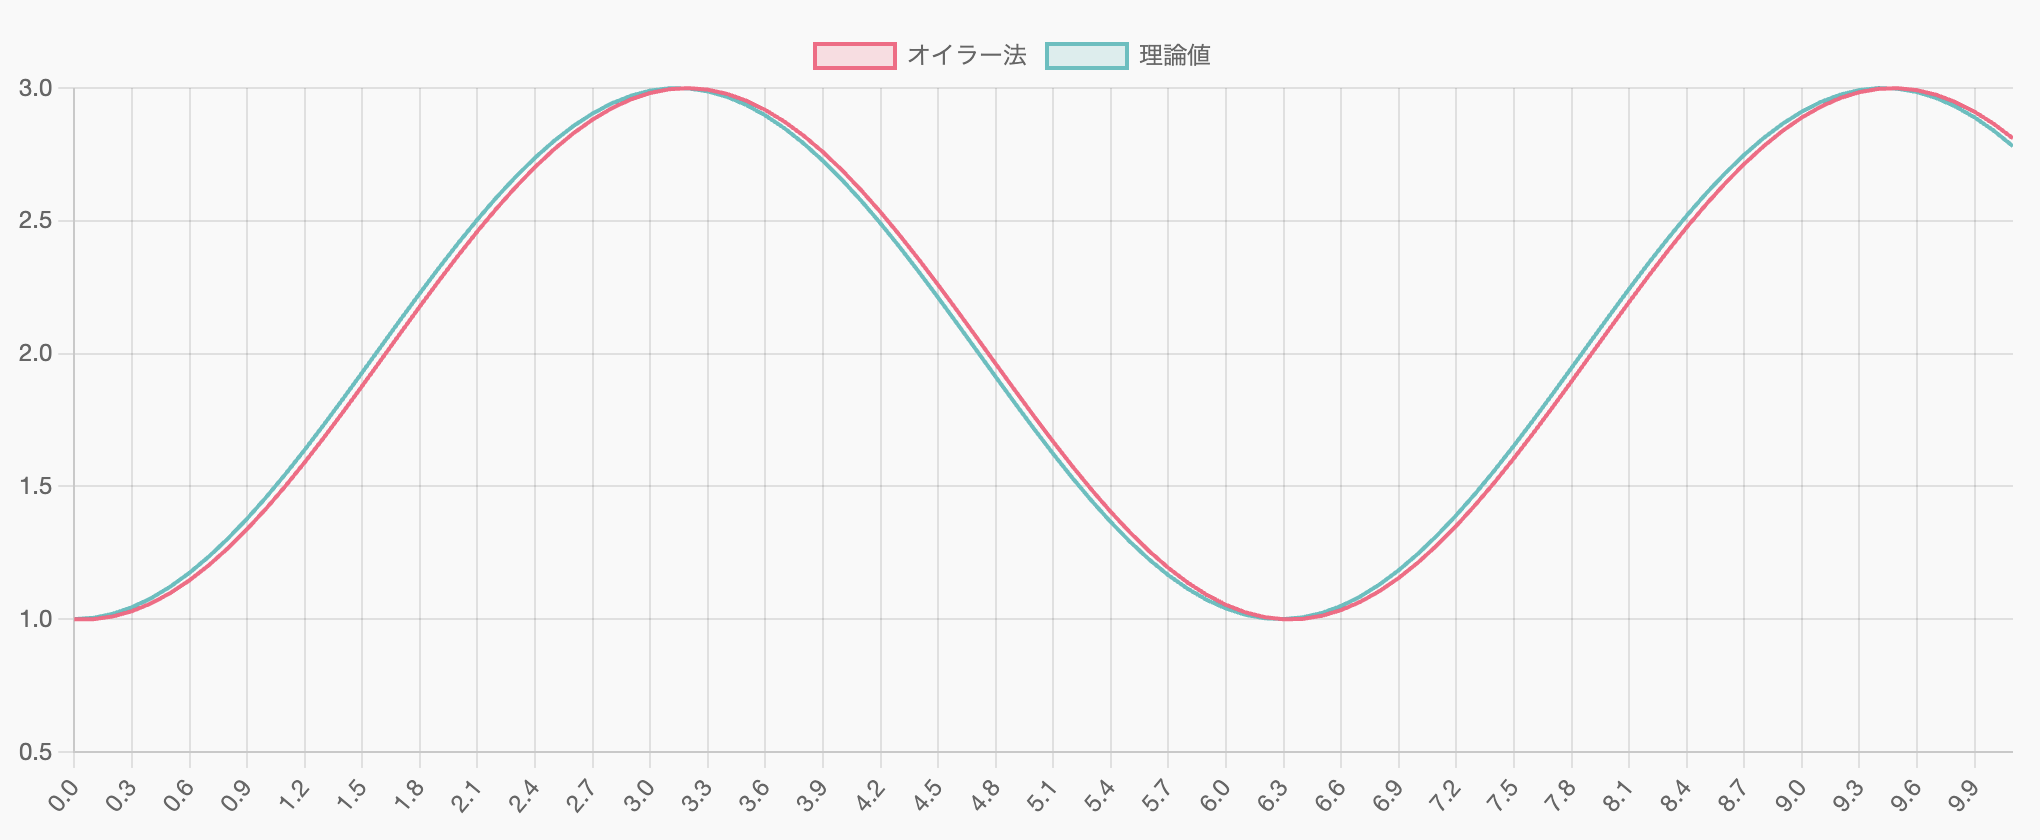
\includegraphics[clip,width=\textwidth,keepaspectratio]{sim-gurafu.png}
\end{center}
\caption{グラフ描画部分}
\label{fig:グラフ描画部分}
\end{figure}

\clearpage

\subsubsection{拡大グラフ描画部分}
拡大グラフ描画部分を図\ref{fig:拡大グラフ描画部分}に示す.拡大グラフ描画部分は計算が完了すると,誤差が最大となる$x$を中心として前後の微小区間5つ分を拡大したグラフを描画する.誤差が小さい際に,グラフ描画部分では視認できない誤差を可視化することができる.また,Chart.jsの設定はグラフ描画部分と同じオプションを利用している.

\begin{figure}[h]
\begin{center}
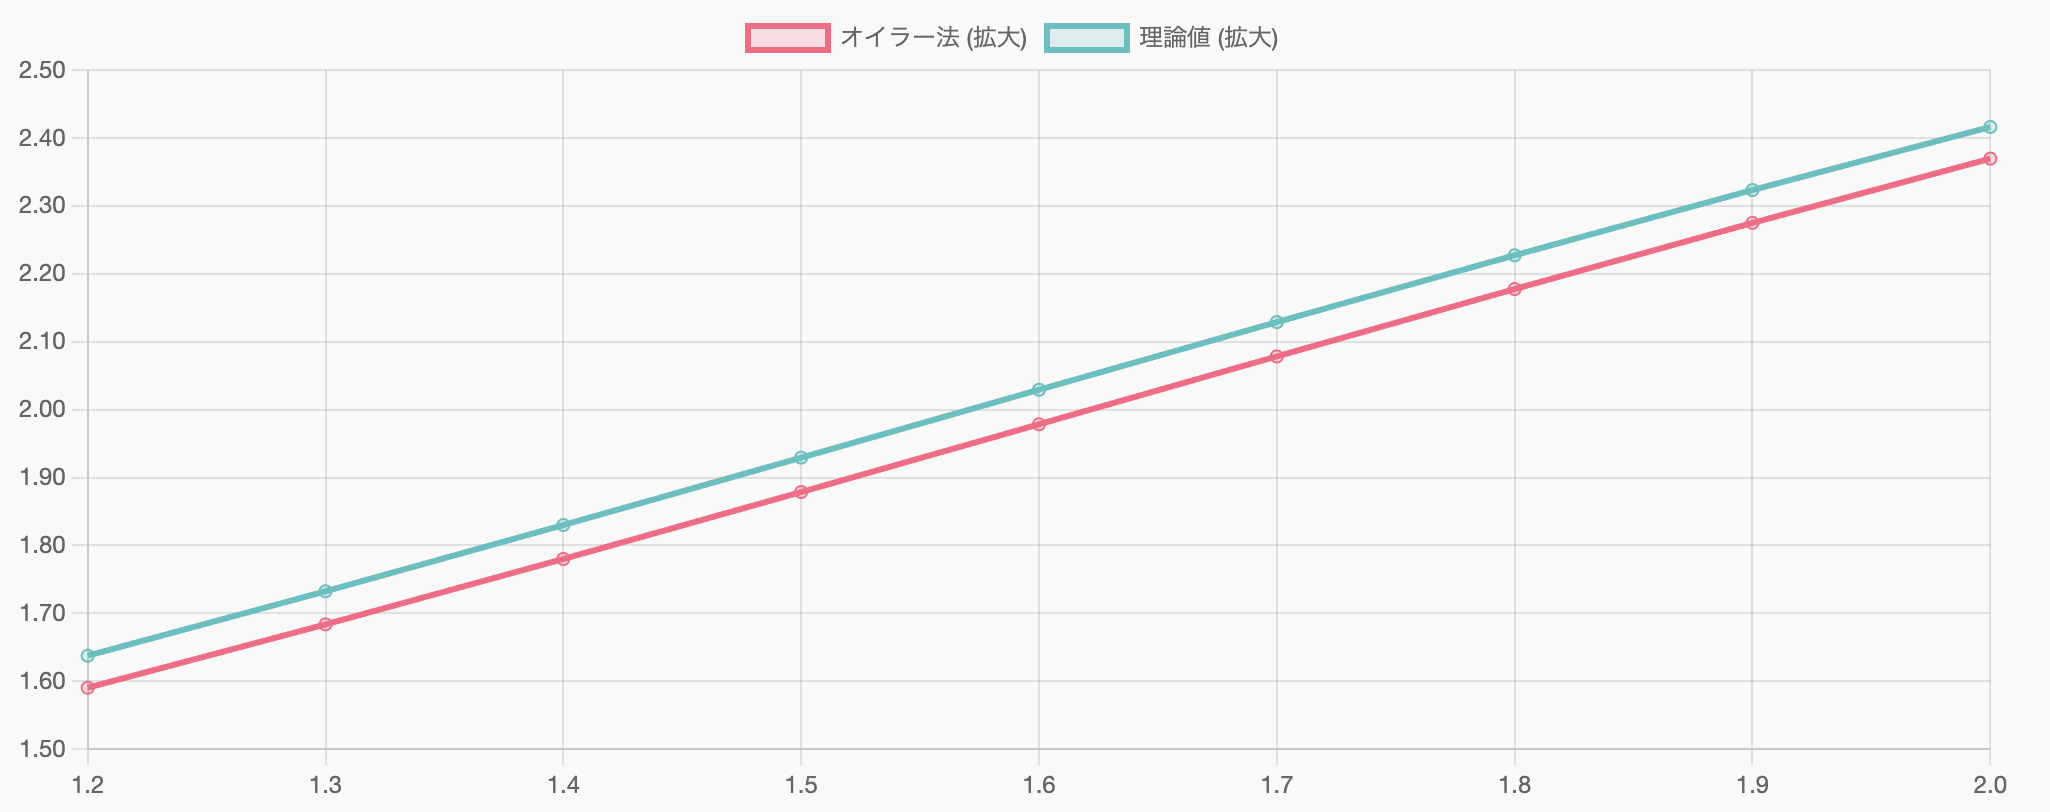
\includegraphics[clip,width=\textwidth,keepaspectratio]{sim-kakudai-gurafu.png}
\end{center}
\caption{拡大グラフ描画部分}
\label{fig:拡大グラフ描画部分}
\end{figure}

\section{評価}
\clearpage
\section{結言}
\clearpage

\bibliography{reference} % 参考文献ファイル名(.bib)
\end{document}